\documentclass[11pt,table]{beamer}
\mode<presentation>
\usepackage{etex}
\usepackage{graphicx}
\usepackage{epstopdf}
\usepackage[english]{babel}
\usepackage{tabularx}
\usepackage{booktabs}
\usepackage{mathrsfs}
\usepackage{multicol}
\usepackage{bm}
\usepackage{subcaption}
\usepackage{wrapfig}
\usepackage{dcolumn}
\usepackage{threeparttable}
\usepackage{booktabs}
\usepackage{bbm}
\usepackage{amsmath,dsfont,listings}
\usepackage{amssymb}
\usepackage{rotating}
\usepackage{multirow}
\usepackage{tcolorbox}
\usepackage[authoryear]{natbib}
\usepackage{circledsteps}
\usepackage{qtree}

\usepackage{tikz}
\usetikzlibrary{arrows,decorations.pathmorphing,backgrounds,fit,positioning,shapes.symbols,chains}
\setbeamertemplate{section in toc}[sections numbered]
\setbeamertemplate{caption}[numbered]

\bibliographystyle{Econometrica}

\setbeamersize{text margin right=3.5mm, text margin left=7.5mm}  % text margin
\setbeamersize{sidebar width left=0cm, sidebar width right=0mm}
\setbeamertemplate{sidebar right}{}
\setbeamertemplate{sidebar left}{}

\definecolor{text-grey}{rgb}{0.45, 0.45, 0.45} % grey text on white background
\definecolor{bg-grey}{rgb}{0.66, 0.65, 0.60} % grey background (for white text)
\definecolor{fu-blue}{RGB}{0, 51, 102} % blue text
\definecolor{fu-green}{RGB}{153, 204, 0} % green text
\definecolor{fu-red}{RGB}{204, 0, 0} % red text (used by \alert)
\definecolor{BrewerBlue}{HTML}{377EB8} % Define Brewer Blue
\definecolor{BrewerRed}{HTML}{E41A1C}  % Define Brewer Red

\setbeamertemplate{frametitle}{%
    \vskip-30pt \color{text-grey}\large%
    \begin{minipage}[b][23pt]{\textwidth}%
    \flushleft\insertframetitle%
    \end{minipage}%
}

\setbeamertemplate{navigation symbols}{} 

%%% begin title page
\setbeamertemplate{title page}{
\vskip2pt\hfill
\vskip19pt\hskip3pt

% set the title and the author
\vskip4pt
\parbox[top][1.35cm][c]{11cm}{\LARGE\color{text-grey} \textcolor{red1}{RL}earning:\\[1ex] \inserttitle \\[1ex] \small \quad \\[3ex]}
\vskip17pt
\parbox[top][1.35cm][c]{11cm}{\small Unit 1-3: \insertsubtitle \\[2ex] \insertauthor \\[1ex]}
}
%%% end title page

%%% colors
\usecolortheme{lily}
\setbeamercolor*{normal text}{fg=black,bg=white}
\setbeamercolor*{alerted text}{fg=fu-red}
\setbeamercolor*{example text}{fg=fu-green}
\setbeamercolor*{structure}{fg=fu-blue}

\setbeamercolor*{block title}{fg=white,bg=black!50}
\setbeamercolor*{block title alerted}{fg=white,bg=black!50}
\setbeamercolor*{block title example}{fg=white,bg=black!50}

\setbeamercolor*{block body}{bg=black!10}
\setbeamercolor*{block body alerted}{bg=black!10}
\setbeamercolor*{block body example}{bg=black!10}

\setbeamercolor{bibliography entry author}{fg=fu-blue}
\setbeamercolor{bibliography entry journal}{fg=text-grey}
\setbeamercolor{item}{fg=fu-blue}
\setbeamercolor{navigation symbols}{fg=text-grey,bg=bg-grey}
%%% end colors

%%% headline
\setbeamertemplate{headline}{
\vskip30pt
}
%%% end headline

%%% footline
\newcommand{\footlinetext}{
%\insertshortinstitute, \insertshorttitle, \insertshortdate
}
\setbeamertemplate{footline}{
\vskip2pt
\hfill \raisebox{-1pt}{\usebeamertemplate***{navigation symbols}}
\hfill \insertframenumber\hspace{10pt}
\vskip4pt
}
%%% end footline

%%% settings for listings package
\lstset{extendedchars=true, showstringspaces=false, basicstyle=\footnotesize\sffamily, tabsize=2, breaklines=true, breakindent=10pt, frame=l, columns=fullflexible}
\lstset{language=Java} % this sets the syntax highlighting
\lstset{mathescape=true} % this switches on $...$ substitution in code
% enables UTF-8 in source code:
\lstset{literate={ä}{{\"a}}1 {ö}{{\"o}}1 {ü}{{\"u}}1 {Ä}{{\"A}}1 {Ö}{{\"O}}1 {Ü}{{\"U}}1 {ß}{\ss}1}
%%% end listings

\usepackage{concmath}
\usepackage{xcolor}
\definecolor{red1}{RGB}{206, 17, 38}
\definecolor{blue1}{RGB}{16, 118, 208}
\definecolor{gray1}{RGB}{117, 115, 115}
\usepackage{hyperref}


\newtheorem{proposition}{Proposition}
\newtheorem{assumption}{Definition}

\title[]{Short guides to reinforcement learning}
\subtitle[]{Upper Confidence Bound}
\author[D. Rostam-Afschar]{\textcolor{gray1}{Davud Rostam-Afschar (Uni Mannheim)}}
\date[]{\today}
\subject{Econometrics}
\renewcommand{\footlinetext}{\insertshortinstitute, \insertshorttitle, \insertshortdate}
\hypersetup{
    bookmarks=false,
    unicode=false,
    pdftoolbar=false,
    pdffitwindow=true,
    pdftitle={Reinforcement Learning for Business, Economics, and Social Sciences: \insertsubtitle},
    pdfauthor={Davud Rostam-Afschar},
    pdfsubject={Reinforcement Learning},
    pdfkeywords={reinforcement learning, Upper Confidence Bound},
    pdfnewwindow=true,
}
\def\sym#1{\ifmmode^{#1}\else\(^{#1}\)\fi}

\begin{document}

\begin{frame}[plain]
  \titlepage
\end{frame}

% --------------------------------------------------- Slide --
%\begin{frame}
	%\frametitle{Content}
	%\tableofcontents[]
%\end{frame}

\section{Upper Confidence Bound}
{
\setbeamercolor{background canvas}{bg=BrewerBlue}
\begin{frame}
\centering
\Huge
\textcolor{white}{How to learn by being optimistic in the face of uncertainty?}
\thispagestyle{empty}
\end{frame}
}


\begin{frame}{Optimism in the Face of Uncertainty}


   Which action should we pick?
				
				\begin{figure}
					\centering
						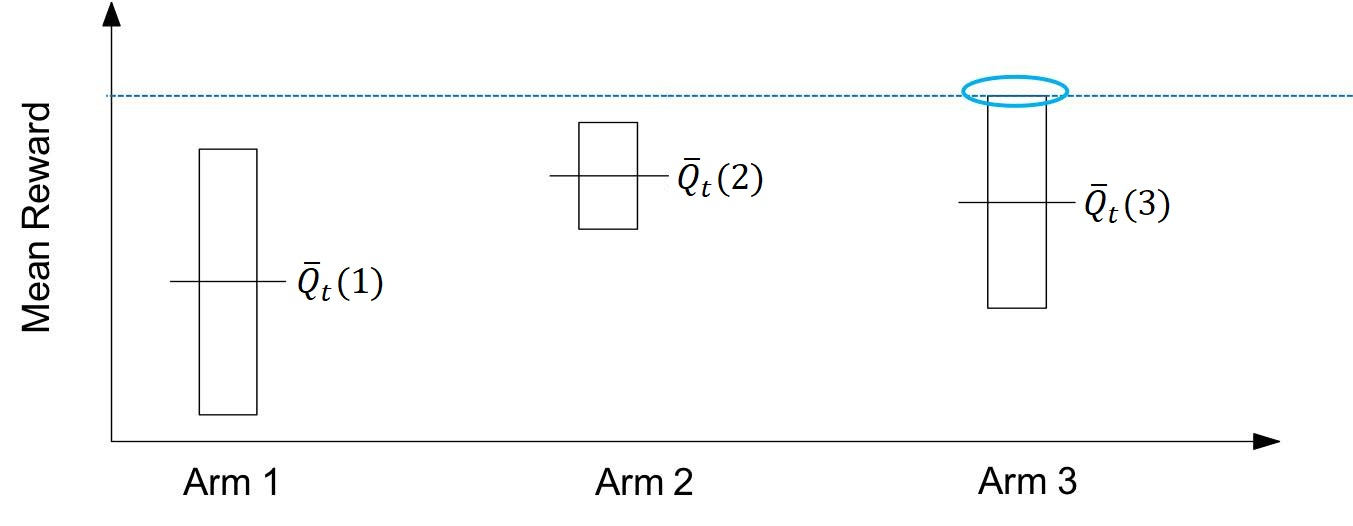
\includegraphics[width=0.60\textwidth]{figures/ucb}
					\label{fig:BOLS}
				\end{figure}
				\only<1>{
        \begin{itemize}
            \item The more uncertain we are about an action-value...
            \item The more important it is to explore that action
            \item It could turn out to be the best action!
        \end{itemize}
				\vspace{2.02cm}}

				\only<2->{
        After picking arm 3:
        \begin{itemize}
            \item We become less uncertain about its value
            \item We are more likely to pick another action
            \item The idea is to always try the best arm\pause\pause, where ``best'' includes\pause
						
						\begin{itemize}
							\item exploitation (average observed reward) and \pause
							\item exploration (uncertainty about observed reward)\pause
						\end{itemize}
						 \citep{auer2002finite}
        \end{itemize}
						}

\end{frame}


\begin{frame}{Convergence}


    \begin{itemize}
        \item  Theorem:\\ An optimistic strategy that always selects $\underset{a}{\operatorname{argmax}} U_t(a)$ will converge to $a^{*}$.\\[2ex]

\item  Proof by contradiction:

\begin{itemize}
\item  Suppose that we converge to suboptimal arm $a$\\ after infinitely many trials\\[2ex]
\item  Then $\overline{Q}(a) =U_{\infty}(a) \geq U_{\infty}(a') =\overline{Q}(a')\quad \forall \ a^{\prime}$\\[2ex]
\item  But $\overline{Q}(a) \geq \overline{Q}(a') \quad \forall \ a^{\prime}$ contradicts our assumption that $a$ is suboptimal\\[2ex]\pause
    \end{itemize}
					\item Problem: We can’t compute an upper bound with certainty since we are sampling
    \end{itemize}
		


\end{frame}


\begin{frame}{Upper Confidence Bounds}
    \begin{itemize}
        \item Estimate an upper confidence $U_t(a)$ for each action value
        \item[] $\Rightarrow$ Such that with high probability
        \[
            q(a) \leq \underbrace{\overline{Q}_t(a)}_{\text{\textcolor{red1}{estimated mean}}} + \underbrace{U_t(a)}_{\substack{\text{\textcolor{red1}{estimated}}\\ \text{\textcolor{red1}{Upper Confidence}}}}
        \]
				\pause
        \item Upper confidence depends on number of times action $a$ has been selected:
        \begin{itemize}
            \item Small $N_t(a)$ $\Rightarrow$ large $U_t(a)$ (estimated value is uncertain)
            \item Large $N_t(a)$ $\Rightarrow$ small $U_t(a)$ (estimated value is accurate)
        \end{itemize}
				\pause
        \item Select action maximizing Upper Confidence Bound (UCB):
        \[
            a_t = \arg\max_{a \in \mathcal{A}} \left[ \overline{Q}_t(a) + U_t(a) \right]
        \]
    \end{itemize}
\end{frame}


\begin{frame}{Hoeffding’s Inequality}
\begin{block}{}
\begin{itemize}
    \item Let $X_1, \ldots, X_t$ be \textit{i.i.d.} random variables in $[0,1]$, and let
    \[
    \overline{X}_t = \frac{1}{t} \sum_{\tau=1}^t X_\tau \quad \text{be the sample mean. Then}
    \]
    \[
    \mathbb{P} \left[ \mathbb{E}[X] > \overline{X}_t + u \right] \leq e^{-2tu^2}
    \]
\end{itemize}
\end{block}

    \begin{itemize}
        \item We will apply \textbf{Hoeffding’s Inequality} to rewards of the bandit\\
              conditioned on selecting action $a$
    \end{itemize}
    
\[
\mathbb{P} \left[ Q(a) > \overline{Q}_t(a) + U_t(a) \right] \leq e^{-2 N_t(a) U_t(a)^2}
\]

\end{frame}

\begin{frame}{Calculating Upper Confidence Bounds}
    \begin{itemize}
        \item Pick a probability $p$ that true value exceeds UCB
        \item Now solve for $U_t(a)$
				
\[
e^{-2 N_t(a) U_t(a)^2} = p
\]

\[
U_t(a) = \sqrt{ \frac{ -\log p }{ 2 N_t(a) } }
\]
\pause
        \item Reduce $p$ as we observe more rewards, e.g.\ $p = t^{-c}, \; c=4$
        \begin{itemize}
            \item (note: $c$ is a hyper-parameter that trades-off explore/exploit)
        \end{itemize}
        \item Ensures we select optimal action as $t \rightarrow \infty$
    \end{itemize}

\[
U_t(a) = \sqrt{ \frac{2 \log t}{N_t(a)} }
\]
\end{frame}


\begin{frame}{UCB: Three-Arm Example for $t = 100$}
\footnotesize
  \begin{table}[h]
    \centering
    \begin{tabular}{c c c c c}
      \toprule
      Arm & Pulls & Empirical mean  & Exploration bonus & $\mathrm{UCB}_a =$ \\
      $a$ & $N_{100}(a)$ & $\overline{Q}_t(a)$ & $\displaystyle \sqrt{\frac{2 \log t}{N_t(a)}}$ & $\overline{Q}_t(a) + \text{bonus}_t(a)$ \\
      \midrule
      1 & 30 & 0.70 & $\sqrt{2\ln(100)/30}=0.554$ & 1.254 \\
      2 & 50 & 0.50 & $\sqrt{2\ln(100)/50}=0.429$ & 0.929 \\
      3 & 20 & 0.60 & $\sqrt{2\ln(100)/20}=0.679$ & 1.279 \\
      \bottomrule
    \end{tabular}
  \end{table}

  \vspace{1em}
  \textbf{Next selection:} Arm 3 (highest UCB of 1.279)
\end{frame}


\begin{frame}{Upper Confidence Bound (UCB)}
    \begin{itemize}
			\item  Choose $a$ with highest Hoeffding bound 
    \end{itemize}

\begin{tcolorbox}[colframe=black, boxrule=1pt, sharp corners]
$\textcolor{red1}{UCB(T)}$

\quad$
Q_t(a) \leftarrow 0, t \leftarrow 0, N_t(a) \leftarrow 0 \quad \forall a
$

\quad Repeat until $t=T$

\qquad$
\text { Execute } \underset{a}{\operatorname{argmax}} \overline{Q}_t(a)+\sqrt{\frac{2 \log t}{N_t(a)}}
$

\qquad Receive $R_t(a)$

\qquad $
Q_t(a) \leftarrow Q_t(a)+R_t(a)
$

\qquad $\overline{Q}_t(a) \leftarrow \frac{N_t(a) \overline{Q}_t(a)+R_t(a)}{N_t(a) +1}$

\qquad $t \leftarrow t+1, N_t(a) \leftarrow N_t(a)+1$

Return $Q_t(a)$

\end{tcolorbox}
    
\end{frame}



\section{Exploration vs Exploitation}
{
\setbeamercolor{background canvas}{bg=BrewerBlue}
\begin{frame}
\centering
\Huge
\textcolor{white}{Exploration vs Exploitation}
\thispagestyle{empty}
\end{frame}
}

\begin{frame}{Upper Confidence Bound (UCB)}
    \begin{itemize}
        \item A clever way of reducing exploration over time
        \item Estimate an upper bound on the true action values
        \item Select the action with the largest (estimated) upper bound:
        \[
            a_t = \arg\max_a \left[ Q_t(a) + c \sqrt{\frac{\log t}{N_t(a)}} \right]
        \]
        \item where $c > 0$ controls the degree of exploration
    \end{itemize}
						\begin{figure}
					\centering
						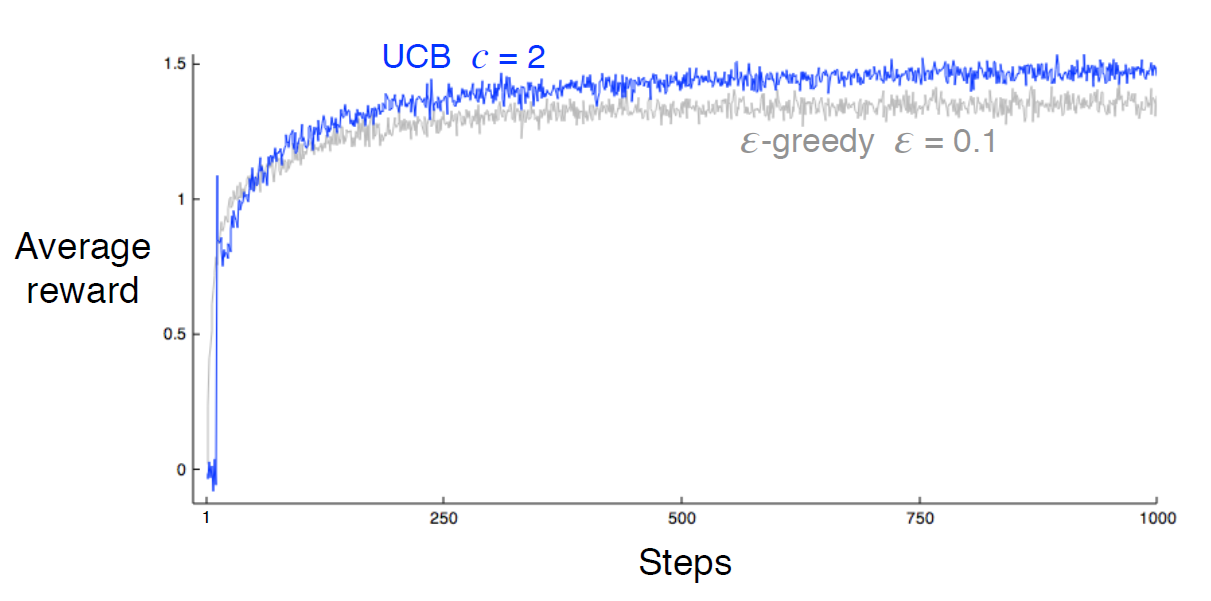
\includegraphics[width=0.60\textwidth]{figures/average reward}
					\label{fig:BOLS}
				\end{figure}
				
\end{frame}




\begin{frame}{UCB Convergence}


    \begin{itemize}
        \item  \textbf{Theorem:} Although Hoeffding's bound is probabilistic, \textcolor{red1}{UCB converges}.

\item  \textbf{Idea:} As $t$ increases, the term $\sqrt{\frac{2 \log t}{N_t(a)}}$ increases, ensuring that all arms are tried infinitely often.\\
The higher $N_t(a)$, the more confident in the estimate for action $a$.

\item  Expected cumulative regret: $\text{Loss}_{T}=\mathcal{O}(\log T)$
\begin{itemize}
    \item \textcolor{red1}{Logarithmic regret} 
    \end{itemize}
    \end{itemize}
\end{frame}




\begin{frame}[t,allowframebreaks
]%\nocite{*}
\frametitle{References}
\small
\bibliography{bib}
\end{frame}



\section{Takeaways}
{
\setbeamercolor{background canvas}{bg=BrewerBlue}
\begin{frame}
\centering
\Huge
\textcolor{white}{Takeaways}
\thispagestyle{empty}
\end{frame}
}

\begin{frame}{What is Upper Confidence Bound (UCB)?}
\begin{itemize}
    \item Uses a probabilistic upper bound to guide action selection
    \item At each step, select action with highest empirical mean plus exploration bonus
    \item Ensures that all actions are tried enough times
		\item It and converges to the optimal arm
    \item Achieves logarithmic regret
		\item UCB often outperforms $\varepsilon$-greedy strategies in practice
\end{itemize}
\end{frame}


\end{document}
